% -*- mode:LaTex; mode:visual-line; mode:flyspell; fill-column:75-*-

\chapter{Programmable In-situ Stiffness Modulation for Efficient Aquatic Robot Locomotion (PISM)}
\label{chapPISM}

\section{Overview}
\label{sec:PISM_overview}

\subsection{Motivation and Contributions}

Fish achieve exceptional propulsive performance across a range of swimming speeds and gait modalities~\cite{lucas_bending_2014, daniel_flexible_2002, dewey_scaling_2013}. Among these widely observed modes are body-caudal-fin (BCF) undulation~\cite{cromie_lear_biomechanical_2020} and drag-based pectoral-fin locomotion~\cite{boudrias_are_2002} for fast swimming and low-speed maneuvering, respectively. A commonality across both swimming modalities is the active modulation of the body's mechanical properties, especially stiffness, to improve swimming performance. For example, fast-swimming tuna and mackerel activate both their axial and caudal-peduncle muscles to stiffen their proximal appendages to achieve high acceleration~\cite{cromie_lear_biomechanical_2020,boudrias_are_2002} while also controlling the distal stiffness to improve vortex-shedding timing at the fin's trailing edge~\cite{hemmati_effects_2019, nedic_vortex_2015}. In contrast, the slower-moving bluegill sunfish actively modulates the compliance of its pectoral fins: stiffening the fin during the power stroke to generate more thrust while softening it during recovery to reduce drag~\cite{floryan_distributed_2020,long_stiffness_1992}. These intricate spatial and temporal stiffness adjustments found in biology may offer a promising blueprint for improving the performance of robotic swimmers~\cite{domenici_kinematics_1997}.

Despite these substantial biomechanics studies of nature's swimmers~\cite{behbahani_design_2016,jia_energy-efficient_2015,hu_design_2024,lu_development_2022,john_h_long_importance_1996}, dynamic stiffness modulation remains comparatively underexplored for robotics~\cite{obayashi_online_2025}, which we largely attribute to the limitations of current mechanisms. Several variable-stiffness approaches have been proposed~\cite{obayashi_online_2025,zhong_tunable_2021,liao_fast_2024,wang_design_2025,wolf_fish-like_2020,sharifzadeh_curvature-induced_2021, kwak_development_2023, Bobing_Octopus_2025}, but each lacks at least one capability used by biological systems: (i) time-varying control of stiffness over a wide range; (ii) spatial programmability across joints or fin rays; and (iii) ease of integration for untethered operation. Specifically, shape memory alloys (SMAs) integrate readily but exhibit thermal buildup and slow response times of up to $\sim$36~seconds~\cite{liu_tunable_2023}; pneumatic or hydraulic systems switch quickly but require external pressure sources, imposing prohibitive payloads for underwater robots~\cite{jusufi_undulatory_2017,obayashi_online_2025,HVS_2023}; spring or elastic-beam designs are limited to single, static stiffness~\cite{zhong_tunable_2021,liao_fast_2024,wang_design_2025,sharifzadeh_curvature-induced_2021}. In addition, systematic optimization for time-varying stiffness remains underdeveloped: most models assume stiffness is time-invariant and therefore do not compute optimal stiffness profiles over a full stroke~\cite{Bobing_Octopus_2025}. A mechanism that can meet all three capabilities may lead to more efficient robotic swimmers.

To address these limitations, this chapter presents a \textbf{programmable in-situ stiffness modulation (PISM)} framework for aquatic robots. The hardware embodiment of this framework is a \textbf{PISM mechanism}, a modular multi-joint arm with sliding laminate flexures at each joint for stiffness tuning. By shifting the insertion depth of a flexure, the corresponding joint stiffness can be changed in under 0.15~s, and different joints can be designed to operate over different stiffness ranges via reconfiguration of the flexure geometry. We further leverage this controllability to perform trajectory optimization for various swimming gaits. The resulting PISM strategy improves propulsion performance over non-programmable baselines by up to 89\% for drag-based swimming and 19\% for body-caudal-fin (BCF) propulsion. These gains are further validated on an untethered, fish-inspired robotic swimmer capable of both BCF and pectoral-fin swimming.

\begin{figure*}[!t]
    \centering
    \includegraphics[width=\linewidth]{figs/spatio/Figure2_v14.pdf}
     \caption{Different bio-inspired swimming modalities considered in this chapter. (a) We study BCF swimming and drag-based pectoral-fin propulsion. BCF involves a fish-like undulation over one period, $T{=}1/f$, while drag-based swimming involves asymmetric ``rowing'' strokes. To enable comparisons across gait frequencies, the cycle is shown using normalized phase $t/T$ (reported as 0--100\% of the period). (b) While many prior robotic systems demonstrate only one of these modalities, the proposed PISM framework is studied for both BCF and drag-based swimming.}
    \label{fig:stifin_lit}
\end{figure*}

The main contributions of this chapter are summarized as follows:
\begin{itemize}
    \item A programmable in-situ stiffness modulation framework for aquatic locomotion, physically realized through a modular multi-link PISM with controllable joint stiffnesses.
    \item A variational-mechanics-based dynamics model and trajectory-optimization framework that use joint-level stiffness trajectories as decision variables for efficient swimming.
    \item Experimental validation on both fixed-base thrust tests and an untethered robotic swimmer, demonstrating the benefits of programmable joint-specific stiffness modulation across multiple swimming modalities.
\end{itemize}

\subsection{Chapter Organization}

The remainder of this chapter is organized as follows. Section~\ref{sec:PISM_mechanism} introduces the PISM hardware and its implementation. Section~\ref{sec:PISM_modeling} presents the variational mechanics model used for simulation and optimization. Section~\ref{sec:PISM_characterization} characterizes joint stiffness, response time, and the correspondence between simulation and hardware morphology. Section~\ref{sec:PISM_optimization} formulates the stiffness-optimization problem for efficient swimming. Section~\ref{sec:PISM_experiments} presents propulsion experiments for drag-based swimming, BCF swimming, and untethered locomotion. Finally, Section~\ref{sec:PISM_discussion} discusses the physical interpretation, limitations, and implications of the proposed framework.

\section{PISM: Mechanism Design and Implementation}
\label{sec:PISM_mechanism}

\subsection{Mechanism Design}

\begin{figure}[!t]
    \centering
    \includegraphics[width=0.6\textwidth]{figs/spatio/Figure1_v21.pdf}
     \caption{A system overview of the programmable in-situ stiffness modulation (PISM) mechanism, which serves as the hardware embodiment of the proposed PISM framework. (a) Side view of PISM. (b) The PISM is a three-layer, modular, multi-joint arm. The top and bottom layers are rigid-link frames (gray). The middle layer contains sliding-laminate flexures (red), a rigid linear guide or constraint (green) that limits the slider to one-degree-of-freedom translation, and passive joints (purple) that define the revolute axes. Each joint can employ a different laminate geometry to realize a different stiffness range. (c) Joint stiffness modulation of the PISM, where a flexure linearly translates across the joint to bring it from a ``flexible'' state to a ``stiff'' state. (d) Top view. Integration of the PISM in an untethered, fish-inspired swimmer that can perform both body-caudal-fin (BCF) and pectoral-fin (drag-based) locomotion.}
    \label{fig:stifin_overview}
\end{figure}

To realize dynamic stiffness modulation, we introduce the PISM, which provides time-varying, joint-specific stiffness with simple actuation. The design details are shown in Fig.~\ref{fig:stifin_overview}b. The hardware is a modular multi-joint arm with sliding laminate flexures at each joint; the flexure's tapered geometry allows for linear translation to modulate the joint stiffness, as illustrated in Fig.~\ref{fig:stifin_overview}c. Each flexure geometry can be further reshaped to tune the stiffness profile of the corresponding joint.

The PISM employs two servomotors. Servo~1 actuates the entire mechanism to follow a swimming gait, while Servo~2 drives a gear rack that linearly translates the sliding flexure. In the prototype used in this chapter, Servo~1 is a HobbyPark Waterproof 45kg High Torque Servo and Servo~2 is an Injora 9kg Servo. This mechanism achieves a wide tuning range and fast retuning, supporting real-time stiffness modulation across diverse bio-inspired gaits and frequencies.

\subsection{Joint Stiffness Modulation}

A key feature of the PISM is that the stiffness of each joint is controlled in situ by changing the effective cross-sectional moment of inertia of a sliding laminate flexure. This design allows the same mechanism to realize both time-varying control and joint-specific stiffness scheduling. Because different flexure geometries can be assigned to different joints, the mechanism also supports spatially heterogeneous stiffness ranges. In other words, the PISM framework is implemented not by a single global compliance adjustment, but by independently programmable local stiffness changes distributed across the mechanism.

This capability is particularly important for aquatic propulsion. In drag-based paddling, different phases of the stroke benefit from different local compliance to enlarge projected area during the power stroke and reduce drag during recovery. In BCF swimming, different joints along the body and tail play distinct roles in transmitting bending waves and setting the trailing-edge amplitude. The PISM therefore provides a hardware substrate that is well matched to these spatially and temporally varying requirements.

\subsection{Fabrication and System Integration}

The modular design allows additional passive joints and links to be added as needed. Throughout this chapter, we use a four-link, three-joint implementation of the PISM. The mechanism is integrated both in a fixed-base propulsion testbed and in an untethered fish-like robotic platform. In the untethered platform, three PISM modules are used: a pair of left--right symmetric pectoral modules for drag-based paddling and a caudal module for BCF propulsion, as shown later in Fig.~\ref{fig:swimmer}.

In practice, the sliding-laminate architecture is also straightforward to fabricate and reconfigure. This is useful both for experimental iteration and for inverse design: once an optimal stiffness schedule is found computationally, a laminate geometry can be designed to realize the desired stiffness range for a particular joint. Fabrication details and dimensional specifications can be placed in the appendix of the thesis if desired.

\section{Variational Mechanics Modeling}
\label{sec:PISM_modeling}

\subsection{System Description and Coordinates}

We model the PISM as a serial chain of $n$ rigid links connected through variably stiff revolute joints, operating in a two-dimensional fluid environment. All symbols used in this section are summarized in Table~\ref{tab:params}. Each link $i \in \{1, 2, \ldots, n\}$ is characterized by length $l_i$, width $w_i$, mass $m_i$, and moment of inertia $J_i$. Each joint $j \in \{1, 2, \ldots, n-1\}$ is characterized by a time-varying stiffness.

We define the system configuration in maximal coordinates:
\begin{equation}
\mathbf{q} = [\mathbf{r}_1^T, \theta_1, \mathbf{r}_2^T, \theta_2, \ldots, \mathbf{r}_n^T, \theta_n] \in \mathbb{R}^{3n},
\end{equation}
where $\mathbf{r}_i = [x_i, y_i]^T$ denotes the center-of-mass position of link $i$, and $\theta_i$ represents its orientation. The corresponding system velocity is defined as $\mathbf{v} = \dot{\mathbf{q}} \in \mathbb{R}^{3n}$.

\begin{table}[t]
  \caption{List of symbols used in the dynamics model}
  \label{tab:params}
  \centering
  \small
  \renewcommand{\arraystretch}{1.1}
  \begin{tabular}{@{}p{2.4cm}p{5.8cm}@{}}
    \hline
    \textbf{Symbol} & \textbf{Physical Meaning} \\
    \hline
    $N$, $L_i$ & Number of rigid links, length of link $i$ \\
    $q=[x_i,y_i,\theta_i]_{i=1}^{N}$ & Generalized coordinate vector \\
    $(x_i,y_i)$, $\theta_i$ & Centroid position and yaw of link $i$ \\
    $c(q)=0$, $J_c$ & Constraint equation, constraint Jacobian \\
    $m_i$, $J_i$ & Rigid mass and planar inertia of link $i$ \\
    $\rho$, $A_i$, $I_i$ & Density, projected area, and polar moment \\
    $C_{am}$, $C_{a\theta}$ & Added-mass and added-inertia coefficients \\
    $m_{ai}$, $J_{ai}$ & Added mass and inertia of link $i$ \\
    $M(q)$ & Total mass matrix \\
    $T$ & Kinetic energy ($\frac{1}{2}\dot{q}^{\mathrm{T}}M\dot{q}$) \\
    $\phi_i$ & Relative joint angle ($\theta_i-\theta_{i-1}$) \\
    $k_i(t)$, $K(k(t))$ & Joint stiffness, equivalent stiffness matrix \\
    $D$ & Joint-difference matrix \\
    $U(q,t)$ & Elastic potential energy \\
    $C(q,\dot{q})$ & Coriolis--centrifugal matrix \\
    $Q_d(q,\dot{q})$ & Quadratic hydrodynamic drag force \\
    $C_d$ & Block-diagonal drag-coefficient matrix \\
    $A_{\text{proj}}$ & Wetted projection area of a link \\
    $B$, $\tau$ & Torque-to-force mapping matrix, joint torques \\
    $\lambda$ & Lagrange multipliers enforcing $c(q)=0$ \\
    $\Delta t$ & Discrete time step \\
    $L_d(q_k,q_{k+1})$ & Discrete Lagrangian \\
    $v_{k+\frac{1}{2}}$ & Mid-interval velocity $(q_{k+1}-q_k)/\Delta t$ \\
    $D_1$, $D_2$ & Discrete variational derivatives \\
    $Q^{\text{nc}}_k$ & Non-conservative force at node $k$ \\
    \hline
  \end{tabular}
\end{table}

\subsection{Principle of Least Action}

We model the PISM using the principle of least action, which formulates the dynamics as a continuous-time optimization problem:
\begin{mini}|l|
  {q,v}{\int_{t_0}^{t_f} T(q,v) - U(q) + F(t)^T q(t)\, dt}{}{}
  \label{eq:la_principle}
  \addConstraint{v = \dot{q},}
  \addConstraint{c(q) = 0,}
\end{mini}
where $q(t) \in \mathbb{R}^{3n}$ is the configuration of the system as a function of time $t$; $v(t) \in \mathbb{R}^{3n}$ is the velocity; $T(v)$ is the kinetic energy of the system; $U(q)$ is the potential energy; and $v=\dot{q}$ represents the kinematic constraint. $F(t)$ represents external, non-conservative forces that are incorporated via the Lagrange--d'Alembert principle of virtual work~\cite{izadi_rigid_2014}. The term $c(q)$ encodes the holonomic constraints, such as the joint constraints between links.

We define the kinetic and potential energies of the PISM as
\begin{align}
    T(v) & = \frac{1}{2} v^T M v, \label{eq:kinetic_energy} \\
    U(q) & = \frac{1}{2} q^T K(t) q, \label{eq:porential_energy}
\end{align}
where $M \in \mathbb{R}^{3n \times 3n}$ is the mass matrix and $K(t) \in \mathbb{R}^{3n \times 3n}$ is the stiffness matrix that encodes the time-varying torsional stiffness at the joints.

\subsection{Variable Stiffness as Control}

The slidable laminate mechanism modulates joint stiffness through controlled adjustment of the effective cross-sectional moment of inertia. The instantaneous stiffness at joint $j$ is written as
\begin{equation}
k_j(u_j(t)) = k_j^{\min} + (k_j^{\max} - k_j^{\min})\sigma(u_j(t)),
\end{equation}
where $u_j(t) \in [0,1]$ is the normalized control input and $\sigma(\cdot)$ is a smooth activation function accounting for laminate overlap dynamics.

The elastic potential energy stored in the compliant joints is
\begin{equation}
V(\mathbf{q}, \mathbf{u}(t)) = \frac{1}{2}\sum_{j=1}^{n-1}k_j(u_j(t))(\theta_{j+1} - \theta_j)^2.
\end{equation}

This can be expressed in matrix form as
\begin{equation}
V = \frac{1}{2}\mathbf{q}^T\mathbf{K}(t)\mathbf{q},
\end{equation}
where $\mathbf{K}(t) = \mathbf{D}^T\mathbf{K}_s(\mathbf{u}(t))\mathbf{D}$ is the time-varying generalized stiffness matrix. In this way, stiffness enters the model as a programmable control variable rather than a fixed structural property.

\subsection{Hydrodynamic Forces}

We model the hydrodynamic forces acting on the PISM using the quasi-steady blade element model~\cite{najafi_numerical_2017}. The drag force on link $i$ is decomposed into normal and tangential components:
\begin{equation}
\mathbf{F}_{d,i} = -\frac{1}{2}\rho l_i w_i
\left[
C_{d,n}(\mathbf{v}_{n,i} \cdot \hat{\mathbf{n}}_i)\hat{\mathbf{n}}_i +
C_{d,t}(\mathbf{v}_{t,i} \cdot \hat{\mathbf{t}}_i)\hat{\mathbf{t}}_i
\right],
\end{equation}
where $\hat{\mathbf{n}}_i$ and $\hat{\mathbf{t}}_i$ are the normal and tangential unit vectors, and $C_{d,n}$ and $C_{d,t}$ are the respective drag coefficients. Meanwhile, the hydrodynamic moment about the link's center of mass accounts for both pressure and friction:
\begin{equation}
\tau_{h,i} = -\frac{1}{12}\rho w_i l_i^3
\left[
C_{d,n}\dot{\theta}_i|\dot{\theta}_i| + C_f\dot{\theta}_i
\right],
\end{equation}
where $C_f$ represents the rotational friction coefficient. These hydrodynamic forces and moments are incorporated into the least-action framework of \eqref{eq:la_principle} as external forces $F(t)$.

\subsection{Joint Constraints}

While the objective of \eqref{eq:la_principle} encodes the dynamics of each individual link of the PISM, we encode the revolute joints between links as holonomic constraints $c(q)=0$. Each revolute-joint constraint is defined as
\begin{equation}
\mathbf{c}_{i+1}(\mathbf{q}) =
\mathbf{r}_i + \frac{l_i}{2}\hat{\mathbf{e}}_i
- \mathbf{r}_{i+1} + \frac{l_{i+1}}{2}\hat{\mathbf{e}}_{i+1}
= \mathbf{0},
\label{eq:joint_constraint}
\end{equation}
where $\hat{\mathbf{e}}_i = [\cos\theta_i, \sin\theta_i]^T$ is the unit vector along link $i$.

We additionally add the following constraint to the first link to simulate a fixed base at the origin:
\begin{equation}
\mathbf{c}_1(\mathbf{q}, t) =
\mathbf{r}_1 - \frac{l_1}{2}[\cos\theta_1, \sin\theta_1]^T = \mathbf{0}.
\label{eq:fixed_base_constraint}
\end{equation}

To model prescribed flapping trajectories, we constrain the angle of the first link, $\theta_1$, to follow a reference trajectory $\theta_{\text{ref}}(t)$:
\begin{equation}
c_{\text{ref}}(q; \theta_{\text{ref}}) =
\theta_1 - \theta_{\text{ref}}(t) = \mathbf{0},
\label{eq:reference_traj_constraint}
\end{equation}
where $\theta_{\text{ref}}(t)$ is designed to simulate specific swimming gaits such as BCF undulation and drag-based propulsion.

\subsection{Variational Leap-Frog Integrator}

Using the least-action principle of \eqref{eq:la_principle}, we develop a structure-preserving variational integrator to simulate the PISM in discrete time. First, we discretize the continuous-time action integral using midpoint quadrature. This yields the discretized least-action principle:
\begin{mini}|l|
  {q_k}{\sum_{k=1}^{2} L_{d}(q_{k}, q_{k+1}) + \tfrac{h}{2}F(t_{k} + \tfrac{h}{2})^T (q_k + q_{k+1})}{}{}
  \label{eq:discrete_least_action}
  \addConstraint{c(q_{k}) = 0,}
\end{mini}
where $q_k$ is the configuration at time $t_k$, $h$ is the time step, and $L_{d}(q_{k}, q_{k+1})$ is the discrete Lagrangian:
\begin{equation}
    L_{d}(q_{k}, q_{k+1}) =
    h L\!\left(
    \underbrace{\tfrac{q_k + q_{k+1}}{2}}_{\Bar{q}_{k+1}},
    \underbrace{\tfrac{q_{k+1} - q_k}{h}}_{\Bar{v}_{k+1}}
    \right).
    \label{eq:midpoint_rule}
\end{equation}

We then obtain the discrete Euler--Lagrange equation:
\begin{multline}
    D_{2}L_{d}(q_{k-1}, q_{k}) + D_{1}L_{d}(q_{k}, q_{k+1}) \\
    + h\Bar{F}_{k} + h\lambda_{k}^T D_{1} c(q_k) = 0,
    \label{eq:discrete_euler_lagrange}
\end{multline}
subject to
\begin{equation}
    c(q_{k+1}) = 0,
    \label{eq:discrete_constraint}
\end{equation}
where $\lambda_{k}$ is the dual variable associated with the constraints. The averaged hydrodynamic forces at the midpoint are
\begin{equation}
    \Bar{F}_k = \frac{1}{2}\Big(F(t_k - \tfrac{h}{2}) + F(t_k + \tfrac{h}{2})\Big).
\end{equation}

To express the dynamics in terms of the full state, $x_k = [q_k, \bar{v}_k] \in \mathbb{R}^{6n}$, we evaluate the slot derivatives in terms of $q_k$ and $\bar{v}_k$ to yield
\begin{multline}
    M\bar{v}_{k+1} + \frac{1}{2} h K\bar{q}_{k+1} + h\Bar{F}_{k}
    + h\lambda_{k}^T D_{1} c(q_k) 
    = M\bar{v}_k - \frac{1}{2} hK\bar{q}_k,
    \label{eq:variational_stationarity}
\end{multline}
with
\begin{align}
    q_{k+1} & = q_k + h \bar{v}_{k+1}, \\
    c(q_{k+1}) & = 0.
    \label{eq:variational_constraint}
\end{align}

The system of equations defined by \eqref{eq:variational_stationarity}--\eqref{eq:variational_constraint} can be solved using Newton's method to simulate the dynamics of the PISM. This yields an implicit second-order leap-frog integrator that remains stable under large deformations and time-varying stiffness.

\section{Characterization and Validation}
\label{sec:PISM_characterization}

\subsection{Joint Stiffness Characterization}

\begin{figure*}[t]
    \centering
    \includegraphics[width=\linewidth]{figs/spatio/Figure3_v12.pdf}
     \caption{Characterization of the PISM's joint stiffness and response time. (a) Experimental setup for torsional-stiffness calibration of the joint with the sliding-laminate flexure. (b) Torque--angle measurements at four flexure configurations. The PISM joint achieves a maximum-to-minimum stiffness ratio of \(K_{\max}/K_{\min}=45.7\). Black markers denote theoretical predictions of the analytical model; the mean relative error is \(13.7\%\) and the overall trend matches the measurements. (c) Response times of the PISM joint during stiffness adjustment from an initial stiffness to a target stiffness.}
    \label{fig:stiffnessexp1}
\end{figure*}

For characterization of the modulated torsional stiffness of an PISM joint, we designed a hardware testbed as shown in Fig.~\ref{fig:stiffnessexp1}a. A single PISM joint with its sliding-laminate flexure was mounted on an optical table and aligned coaxially with a torque sensor (ATI Nano17, 6-axis) and a rotary servomotor (XW540-T260). The joint axis, sensor axis, and motor shaft were colinear to avoid parasitic moments. All fixtures were rigidly clamped to eliminate base compliance.

To characterize the flexure's influence on joint stiffness, we performed tests across four equally spaced configurations of the flexure. At each position, the joint was driven quasi-statically through target angles \(\theta \in [0^\circ,\,60^\circ]\) while recording the resulting torque \(\tau(\theta)\). For each slider position, the local torsional stiffness \(K_r\) was estimated from the slope \(d\tau/d\theta\) of a linear least-squares regression over the measured torque data.

The joint exhibits a tunability of \(K_{\max}/K_{\min}=45.7\), as shown in Fig.~\ref{fig:stiffnessexp1}b. This large modulation range spans the stiffness regimes required by both drag-based paddling and BCF undulation over the target flapping band \(0\sim2~\mathrm{Hz}\), enabling the same mechanism to realize both gaits effectively.

To model the resulting joint stiffness as a function of flexure geometry, we use
\begin{equation}
k_t = \frac{E_f I_f}{l_f},
\label{eq:kt_joint}
\end{equation}
where \(E_f\) is the Young's modulus of the in-plane bending layer, \(I_f\) is the second moment of area determined by the flexure's effective width and thickness under a given slider position, and \(l_f\) is the effective bending length.

The measured \((\theta,\tau)\) datasets at four slider locations were used to compute the local torsional stiffness. Independently, the analytical form in \eqref{eq:kt_joint}, together with the geometric relation for \(I_f(\theta)\), yields a nominal stiffness map \(K_s(\theta)\). Over the tested domain, the mean relative error between the model and experiments is \(13.7\%\), indicating sufficient fidelity to guide the design of the flexure geometry.

\subsection{Response-Time Characterization}

To assess the practical use of the PISM for real-time stiffness tuning, we also measured the response time required to transition from an initial joint stiffness to a commanded value, as shown in Fig.~\ref{fig:stiffnessexp1}c. In these tests, the joint was fixed at \(\theta=45^{\circ}\) and step changes were commanded from an initial stiffness \(K_{\text{init}}\) to a target \(K_{\text{target}}\). The response time was defined as the \(0\sim100\%\) transition of the estimated stiffness following the command.

From the calibrated stiffness--position map and the rack--servo kinematics, the two endpoints correspond to servo angles \(\phi_s=0^{\circ}\) and \(60^{\circ}\), so the required travel for any retuning is at most \(60^{\circ}\). We stepped between stiffness setpoints at seven targets uniformly spanning the operable range on hardware \((0\sim343~\mathrm{N{\cdot}mm\,deg^{-1}})\). The measured response times are consistently less than \(0.15~\mathrm{s}\) across the entire operable range of stiffness values. The worst-case mean response time was \(0.147\,\mathrm{s}\), which we attribute to the resulting reaction torque on the servo.

This fast retuning supports stiffness control that static spring or beam designs cannot achieve, while avoiding the latency and payload penalties of SMA and pneumatic or hydraulic approaches~\cite{liu_tunable_2023,jusufi_undulatory_2017,obayashi_online_2025}. It therefore demonstrates the practicality of the proposed in-situ stiffness control for real-time robotic tasks.

\subsection{Morphology and Trajectory Validation}

\begin{figure*}[t]
    \centering
    \includegraphics[width=\linewidth]{figs/spatio/Figure4_v3.pdf}
    \caption{Stiffness--amplitude coupling and morphology across frequency. (a) Soft state. (b) Stiff state. Bottom rows: experimental tip-path envelopes and wakes at 0.1, 1.0, and 2.0~Hz (\(30^\circ\) base amplitude), illustrating the transition in propulsor--flapping coupling---coupling degrades rapidly with frequency in the soft state, whereas the stiff state preserves larger excursions. Top rows: simulations under the same stiffness--frequency conditions reproduce the observed envelopes and sweep-to-figure-eight morphologies, supporting simulator fidelity.}
    \label{fig:stiffnessexp}
\end{figure*}

To simulate the PISM, we utilize variational mechanics to develop a discrete-time dynamics model of the full multibody physics with time-varying joint stiffness. We then compare simulated and empirical tip-path envelopes and morphology of the PISM in the flexible and stiff regimes at 0.1, 1.0, and 2.0~Hz, as shown in Fig.~\ref{fig:stiffnessexp}.

In the flexible state, the envelope contracts sharply with frequency and the trajectory transitions from a broad sweep to a compact figure-eight, indicating degraded propulsor--flapping coupling at high frequencies. In the stiff state, excursions remain large across the frequency sweep, preserving coupling and tip amplitude. The simulator with accurate torsional joint stiffness parameters reproduces these qualitative transitions, the relative amplitude scaling, and the morphology in both stiffness states, including the same sweeping and figure-eight tip trajectories.

This consistency of bending behavior observed on hardware supports the dynamics model's use for trajectory optimization while also highlighting the importance of stiffness modulation in shaping gait behavior.

\section{Optimization of PISM for Efficient Swimming}
\label{sec:PISM_optimization}

\subsection{Problem Setup}

\begin{figure*}[t]
    \centering
    \includegraphics[width=\linewidth]{figs/spatio/Figure5_v4.pdf}
     \caption{Optimization and co-design results for BCF and drag swimming. (a,e) Average simulated thrust force over three cycles with different stiffness-modulation strategies under different control frequencies for the two swimming modes. (b,f) Simulated thrust force and first-link angle over one cycle for drag and BCF swimming modes. (c,g) Optimized stiffness profiles under BCF and drag swimming with different strategies: Opt~$K_{\text{const}}$ = time-invariant, per-joint optimized stiffness (spatial-only); Opt~$TK(t)$ = temporal-only schedule identical across joints (no spatial variation); Opt~$SK(t)$ = joint-specific time-varying stiffness schedule. (d,h) Sliding laminate flexures designed from the optimized stiffness profile under drag and BCF swimming modes. Flapping frequency is 1~Hz in this case.}
    \label{fig:opt}
\end{figure*}

For both BCF and drag-based swimming modes, we formulate a trajectory-optimization problem with average thrust maximization over each period as the objective. Using direct collocation (DIRCOL), we compute joint-specific stiffness schedules of the PISM over a single flapping cycle.

Specifically, we optimize the stiffness trajectory over one swimming-gait period to maximize the net propulsive thrust generated:
\begin{mini}|l|
  {x_{1:N}, K_{1:N}}{\sum_{k}^{N} \underbrace{-p^{T}\lambda_{k}}_{F_{k}^{\text{thrust}}},}{}{}
  \label{opt:trajopt}
  \addConstraint{x_0=x_{\text{init}}}
  \addConstraint{K_0=K_{\text{init}}}
  \addConstraint{f(x_{k+1}, K_{k+1}, x_k, K_k) = 0, \; k = 0, 1, \ldots, N}
  \addConstraint{K_j^{\min} \leq K_{k, j} \leq K_j^{\max}, \; j = 1, \ldots, n-1}
\end{mini}
where $x_{1:N}$ are the states over the trajectory, $K_{1:N} \in \mathbb{R}^{n-1}$ is the joint-stiffness trajectory, and $x_{\text{init}}$, $K_{\text{init}}$ are the initial conditions of the state and joint stiffnesses, respectively. The function $f(\cdot)$ represents the dynamics constraints defined by \eqref{eq:variational_stationarity}--\eqref{eq:variational_constraint}. We additionally enforce stiffness bounds for each joint. Finally, the generated thrust force is equal and opposite to the corresponding reaction force at the fixed-base joint; this scalar is an element of $\lambda_k$ selected by the vector $p$.

\subsection{Gait Parameterization}

These gaits are optimized across a frequency sweep of $0\sim 2.0\,\mathrm{Hz}$, with a consistent base amplitude of \(30^\circ\) for BCF and \(40^\circ\) for drag. For drag mode, we also apply asymmetric flapping by specifying a stroke ratio defined as the fraction of the period allocated to the power stroke:
\begin{equation}
D = \frac{T_{\text{power}}}{T}.
\end{equation}
With \(D=0.4\), the power stroke occupies 40\% of the cycle and is therefore faster than the recovery stroke.

We benchmark the PISM strategy against four non-programmable baselines:
\begin{itemize}
    \item \(K_{\max}\): all joints fixed at their maximum stiffness,
    \item \(K_{\min}\): all joints fixed at their minimum stiffness,
    \item Opt~\(K_{\text{const}}\): a time-invariant stiffness optimized per joint but constant over the cycle (spatial-only),
    \item Opt~\(TK(t)\): a temporal schedule identical across all joints (no spatial variation).
\end{itemize}
Our proposed method, Opt~\(SK(t)\), prescribes a joint-specific time-varying stiffness schedule over each stroke.

Simulation results for thrust optimization under both modalities are shown in Fig.~\ref{fig:opt}a,e, while Fig.~\ref{fig:opt}b,f compares simulated thrust and kinematics at 1~Hz. The corresponding spatial and temporal stiffness distributions are shown in Fig.~\ref{fig:opt}c,g. Finally, based on the characterized stiffness--position mapping in Fig.~\ref{fig:stiffnessexp1}, we inversely design the laminate flexure geometries required to realize the optimized stiffness schedules in hardware.

\subsection{Numerical Solver}

The resulting nonlinear program in \eqref{opt:trajopt} is solved using an interior-point-based method implemented in the MATLAB Optimization Toolbox. Parallel Computing Toolbox is also used to reduce solving time. The optimization solver was run on a system with an 8-core CPU and 32~GB RAM. The average optimization runtime is approximately 1.5~hours.

Overall, the optimized joint-specific time-varying stiffness schedules consistently achieve substantial simulated performance improvements over all baseline methods. These optimized schedules are then translated into realizable hardware commands using the experimentally calibrated stiffness map.

\section{Experimental Results}
\label{sec:PISM_experiments}

\subsection{Experimental Setup}

\begin{figure}[t]
    \centering
    \includegraphics[width=8.0cm]{figs/spatio/Figure6_v4.pdf}
     \caption{Experimental setup for measuring thrust and morphology trajectory of the PISM architecture. Tests are conducted in initially still water for two swimming modalities: BCF and drag-based swimming. (a) Test tank with overhead camera for vision-based motion tracking. The PISM is rigidly mounted to a 1-DOF S-type load cell; reflective markers are attached on top of the PISM. Thrust is sampled at 80\,Hz with an Arduino Uno (calibrated load cell), while an Adafruit Feather M0 commands the flapping motor (Servo~1) and the stiffness motor (Servo~2). (b) Mounting configurations for the two propulsion modes. Because BCF and drag paddling generate thrust along different axes, the load-cell measurement directions are orthogonal. To mitigate tank-wall and recirculation effects, drag tests are aligned with the long axis of the tank, whereas BCF tests use the wide axis.}
    \label{fig:expsetup2}
\end{figure}

To evaluate the use of the PISM for bio-inspired propulsion, we developed a hardware testbed as shown in Fig.~\ref{fig:expsetup2}. The PISM is submerged in a water-filled tank measuring 130\,cm\,(L)$~\times~$80\,cm\,(W)$~\times~$60\,cm\,(H) and fixed to a 0--5\,kg S-type load cell that measures the generated thrust. For all tests, the PISM is oriented accordingly to mitigate wall and recirculation effects. Videos are recorded at 30~FPS and used for vision-based trajectory tracking of the PISM's joint positions. Electrical input power under constant-voltage supply is monitored during the experiments.

To analyze propulsion efficiency, we define the efficiency coefficient as
\begin{equation}
\eta = \frac{\sqrt{\bar{P}^{3}}}{U I_{c}},
\end{equation}
where $U$ denotes the motor voltage, $I_c$ the current, and $\bar{P}$ the static propulsion. A larger $\eta$ reflects greater efficiency in converting electrical input into propulsive output.

\begin{figure*}[t]
    \centering
    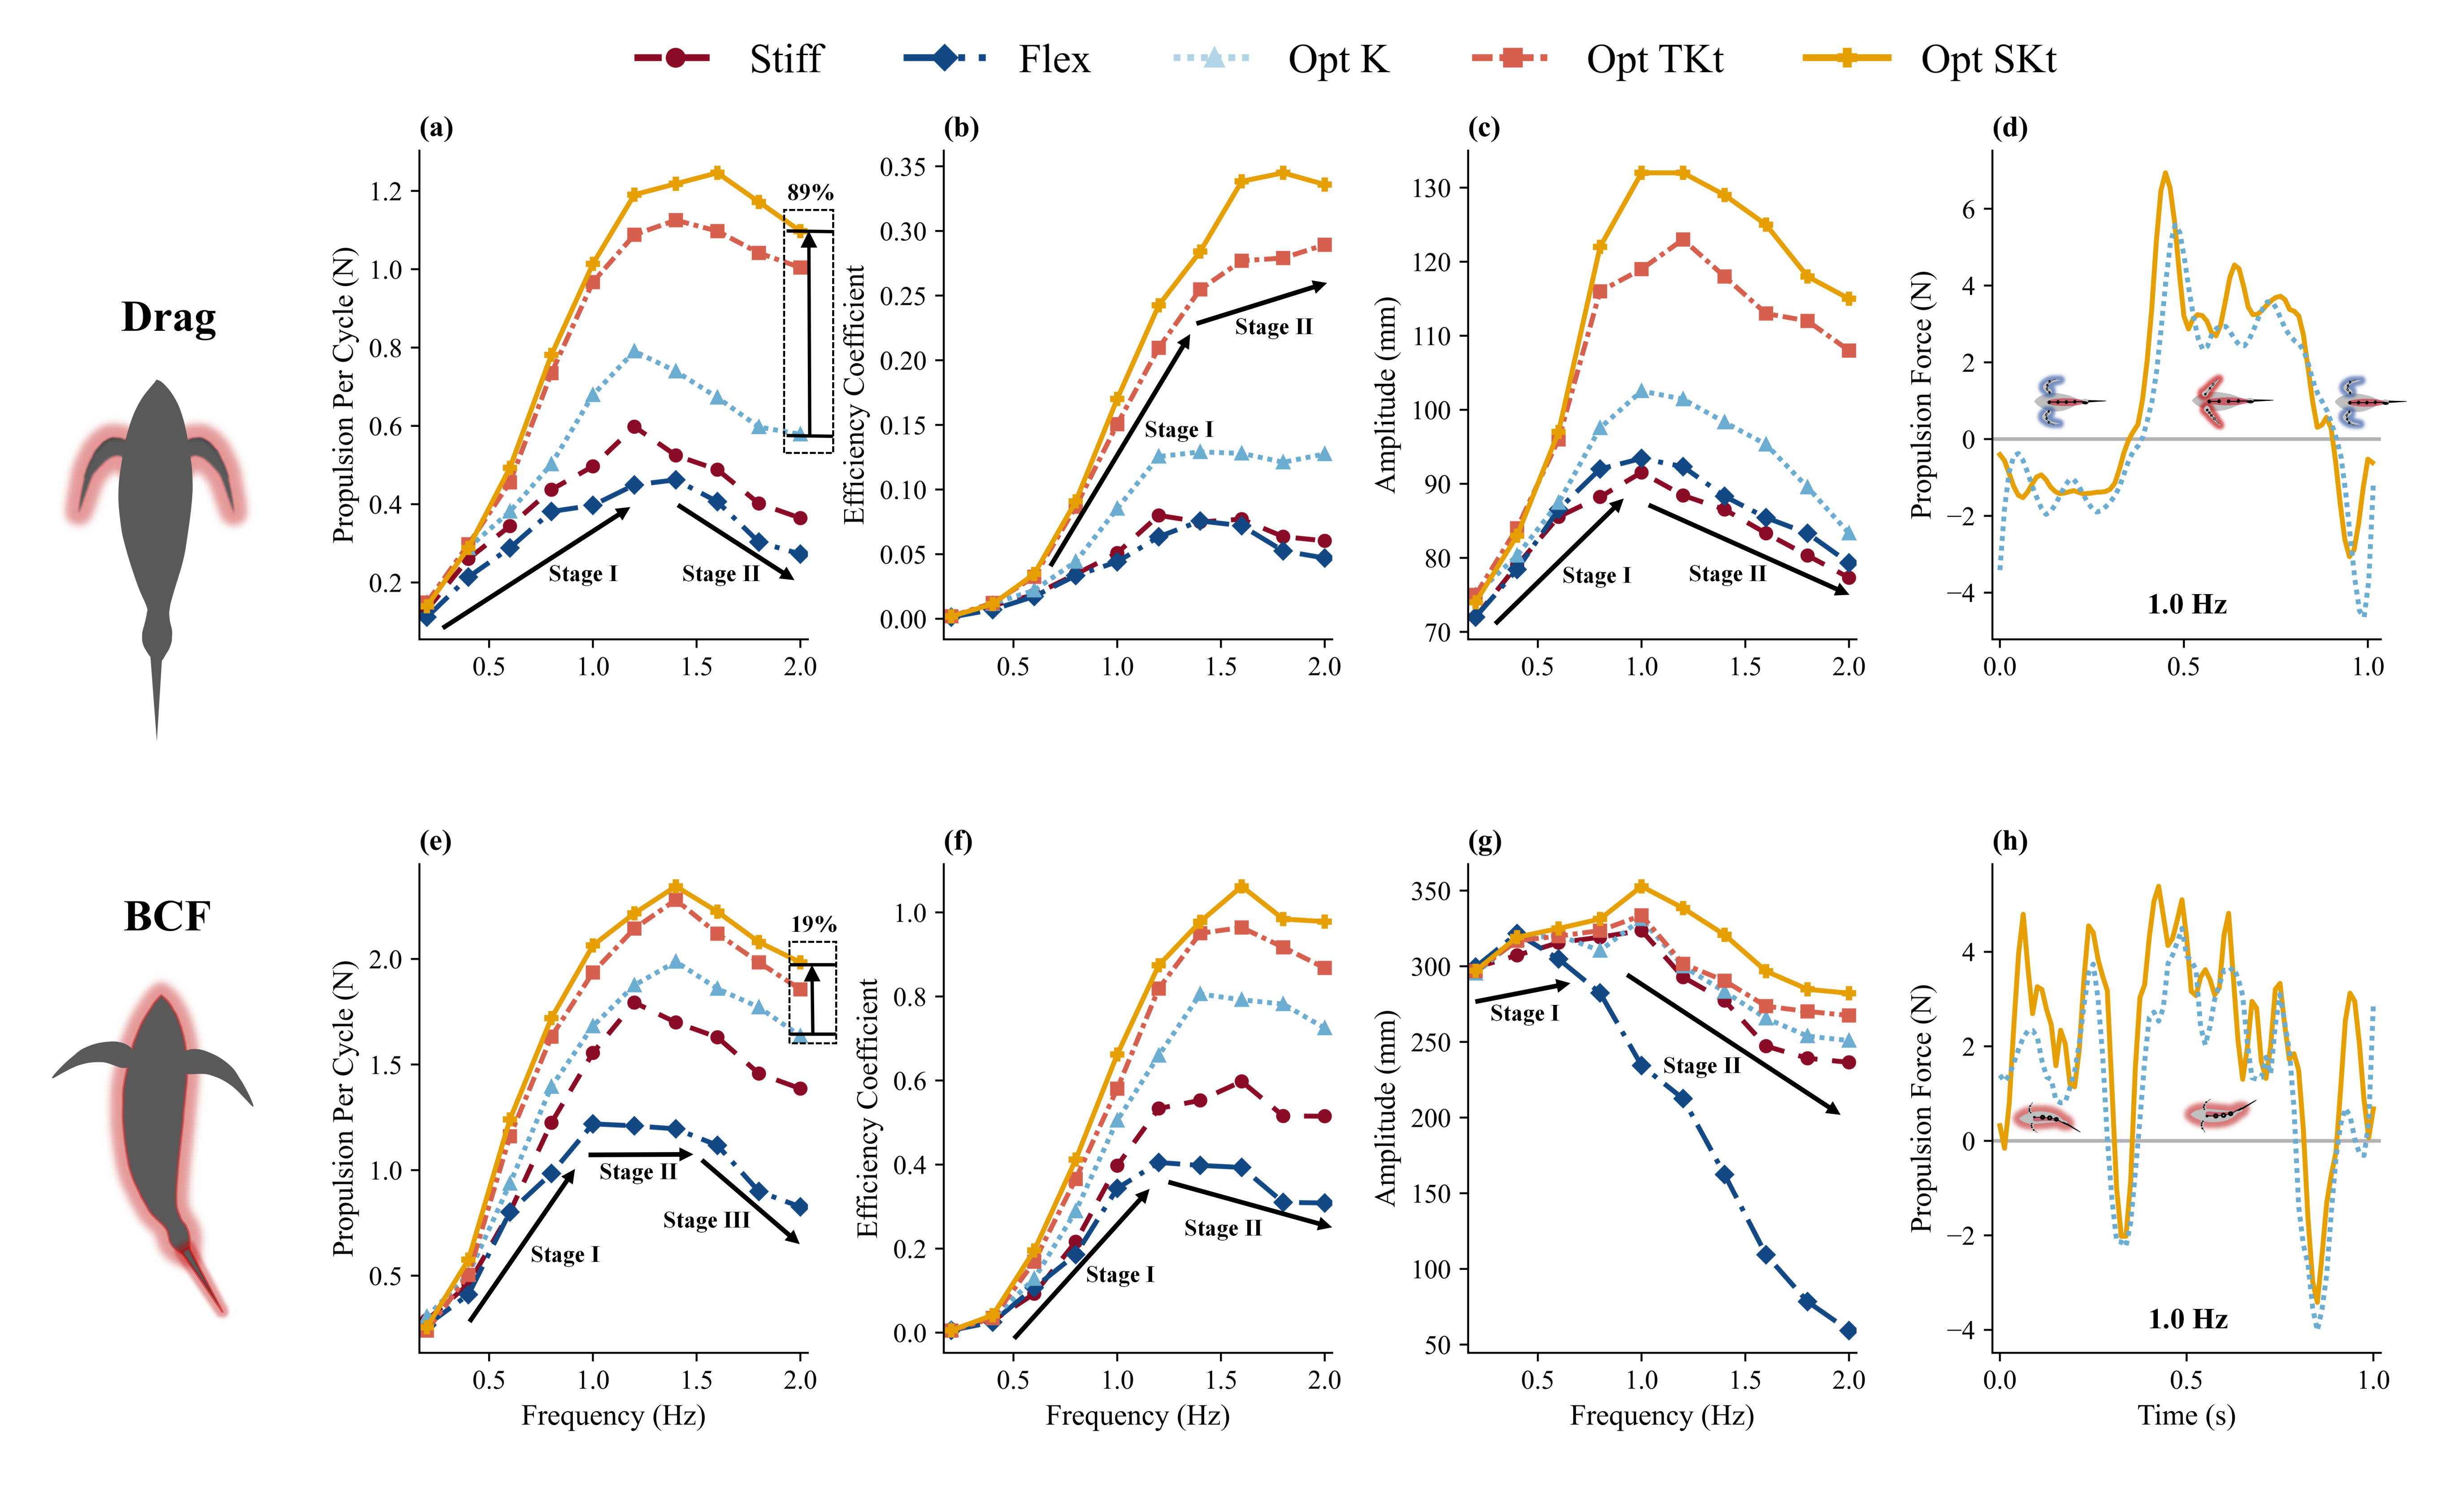
\includegraphics[width=\linewidth]{figs/spatio/Figure7_v7.png}
    \caption{Experimental thrust results of the PISM across various flapping frequencies. (a--c) Cycle-averaged thrust, efficiency coefficient, and tip-path amplitude for a drag-based swimming gait. (d) Time-series propulsion force at $1.0~\mathrm{Hz}$ comparing static and programmable stiffness optimization in drag mode. (e--g) Corresponding plots for the BCF swimming gait. (h) Time-series propulsion force at $1.0~\mathrm{Hz}$ in BCF mode. Error bars denote mean~$\pm$~standard deviation across $n{=}5$ independent trials per frequency and control strategy. Across all frequencies for each swimming modality, Opt~$SK(t)$ consistently outperforms the baselines, with thrust gains of up to $+89\%$ in drag-based swimming and $+19\%$ in BCF undulation relative to the constant-stiffness baseline Opt~$K_{\text{const}}$.}
    \label{fig:force}
\end{figure*}

\subsection{Drag-Based Swimming}

To analyze the propulsive performance of the PISM, we measured the resulting thrust force generated by the optimized gait trajectories on hardware. Across the frequency range, the PISM strategy produces higher thrust than all baselines, with the corresponding efficiency coefficient trend shown in Fig.~\ref{fig:force}a--c.

In the low-frequency regime, thrust rises nearly linearly with frequency for all settings, with a thrust peak near \(1.2~\mathrm{Hz}\); efficiency peaks slightly earlier at \(1.0~\mathrm{Hz}\). As frequency rises further, tip amplitude decreases and baseline thrust rolls off. By coordinating where and when a high stiffness is needed within the stroke, the PISM strategy maintains larger tip amplitude and delays the roll-off. At 2.0\,Hz it yields a \(+89\%\) thrust improvement relative to Opt~\(K_{\text{const}}\) under identical input.

The end-point trajectories in the insets of Fig.~\ref{fig:force}a,c show that, with programmable joint-specific stiffness modulation, propulsor--flapping coupling is preserved as frequency increases, maintaining large tip excursions and delaying amplitude decay. Specifically, the trajectory envelope is wider than that of the spatial-only or temporal-only stiffness control strategies. Spatial-only control does not adapt within the stroke, and temporal-only control lacks spatial specificity. The programmable schedule widens and lengthens the end-point path, thereby increasing the stroke-wise projected-area asymmetry between the power and recovery half-strokes and enhancing the net positive drag thrust.

\subsection{BCF Swimming}

For the BCF gait, the PISM exhibits similar trends in propulsion performance, as shown in Fig.~\ref{fig:force}e--h. The thrust and efficiency peak near 1.4\,Hz, with BCF generating substantially greater thrust than the drag-based gait and slightly higher efficiency. The PISM strategy still improves upon all baselines in both generated thrust and efficiency.

Qualitatively, the generated BCF-undulation trajectory involves a nearly symmetric stiffness profile within one gait cycle. The end-point flapping amplitude shows a brief rise followed by a more nearly linear decline, which is consistent with the simulation results. In addition, programmable stiffness modulation results in a greater trailing-edge amplitude, which coincides with Lighthill's elongated-body theory, where thrust is strongly influenced by the trailing-edge motion~\cite{lighthill_large-amplitude_1997}. The time-series thrust profiles at 1.0\,Hz in Fig.~\ref{fig:force}d,h further illustrate how the optimized stiffness schedule enhances instantaneous thrust generation within each stroke cycle, yielding stronger and more sustained propulsion peaks than the static-stiffness control.

\subsection{Untethered Robot Validation}

\begin{figure*}[t]
    \centering
    \includegraphics[width=0.98\linewidth]{figs/spatio/Figure8_v2.pdf}
\caption{Swimming robot platform and experimental results in drag and BCF swimming gaits. (a) Overview of the fish-like untethered platform integrated with three PISM modules. (b) Hardware configuration of the robot system. (c,d) Displacement of the robot platform under two swimming gaits at different flapping frequencies with the same amplitude. (e,f) Cost of transport (COT) of the robot platform under the two swimming gaits. (g,h) Swimming motion of the robot and PISM morphology in the two swimming modes. Due to small manufacturing variations and initial slider-position offsets, the robot exhibited noticeable yaw deviation during straight swimming, resulting in relatively large COT bounds, especially in the highly deformable Flex mode. All experiments were conducted five times in still water.}
    \label{fig:swimmer}
\end{figure*}

A fish-like robotic platform is used to validate the stiffness-optimization strategies, as shown in Fig.~\ref{fig:swimmer}a. The platform integrates three PISMs: a pair of left--right symmetric pectoral modules for drag-based paddling and a caudal module for BCF propulsion. Each module is mounted to the hull via Heli-Coil inserts. Each PISM comprises a flapping servo and a stiffness-adjustment servo that drives a slider for in-cycle stiffness modulation.

The hull is fabricated via FDM 3D printing and coated with a waterproof layer. All electronics are housed within the hull. A LoRa antenna enables remote control, and an INA219 monitors current in real time to estimate the average electrical power \(P\). Power is supplied by a 7.4\,V Li-Po battery and regulated by a DC--DC converter to independently feed the servos and the microcontroller. The control architecture is shown in Fig.~\ref{fig:swimmer}b.

Experiments were conducted in a $3.0 \times 1.5\,\mathrm{m}$ still-water tank. Vehicle pose was tracked at 30\,Hz using AprilTag to estimate swimming speed. For both BCF and drag gaits, we evaluated the same set of baselines as in the fixed-base thrust tests: Stiff, Flex, Opt~\(K_{\text{const}}\), and Opt~\(TK(t)\), alongside the proposed Opt~\(SK(t)\). For each drive frequency \(f\), we computed the mean swimming speed \(v\) and the cost of transport,
\begin{equation}
\mathrm{COT}=\frac{P}{m g v},
\end{equation}
where \(P\) is the average electrical input, \(m\) is the vehicle mass, and \(g\) is gravitational acceleration. Results are summarized in Fig.~\ref{fig:swimmer}c--f.

Overall trends are consistent with the fixed-base thrust measurements and simulations. BCF generally achieves larger net thrust and higher propulsive efficiency than drag; however, at low frequencies, limited trailing-edge linear velocity suppresses effective BCF thrust, whereas drag benefits from projection-area effects and flapping-frequency asymmetry between power and recovery strokes. As frequency increases, BCF outperforms drag in the 1.0$\sim$2.0\,Hz range, exhibiting higher energetic efficiency and greater per-cycle net thrust.

Different stiffness-modulation strategies are validated under both gaits. Opt~\(SK(t)\) adaptively maintains higher effective thrust and improves swimming efficiency across the full frequency range from 0.2\,Hz to 2.0\,Hz. In drag mode, compared with Opt~\(K_{\text{const}}\), Opt~\(SK(t)\) yields a maximal average-speed gain of \(143.3\%\) at \(f{=}2.0\,\mathrm{Hz}\) while reducing COT by \(34.78\%\); relative to Opt~\(TK(t)\), Opt~\(SK(t)\) is \(18.6\%\) faster at \(2.0\,\mathrm{Hz}\). In BCF, Opt~\(SK(t)\) also surpasses all baselines: compared with Opt~\(K_{\text{const}}\), the largest locomotion improvement occurs at \(f{=}1.5\,\mathrm{Hz}\) and reaches \(19.8\%\). There is also a \(10.2\%\) improvement at \(f{=}2.0\,\mathrm{Hz}\), with a \(25.38\%\) reduction in COT.

These results indicate that static stiffness cannot simultaneously optimize thrust and efficiency over the full frequency band. By contrast, a programmable in-situ stiffness distribution significantly enhances swimming performance, especially at higher frequencies. We further observe that the beneficial morphological effects of the optimized stiffness schedule on the propulsor increase with drive frequency, mirroring the fixed-base morphology and thrust trends reported earlier.

\section{Discussion}
\label{sec:PISM_discussion}

\subsection{Interpretation of Results}

Our results demonstrate that intricate control of stiffness across both time and space can greatly improve bio-inspired propulsion performance. Across a wide gait frequency range ($0\sim 2.0\,\mathrm{Hz}$), the proposed PISM strategy sustains higher thrust and efficiency than time-invariant and spatially invariant baselines across multiple swimming modalities. Specifically, we achieve peak thrust gains of 89\% in drag-based paddling and 19\% in BCF undulation under equivalent voltages.

These performance gains are consistent with the observed morphology. In the drag-based gait, the optimized stiffness schedule enlarges and elongates the end-point envelope compared with static stiffness optimization. This increases the projected-area difference between power and recovery strokes and results in enhanced net thrust generation. For the BCF gait, the trailing-edge amplitude is larger under the optimized stiffness schedule compared with the static-stiffness results, consistent with Lighthill's elongated-body theory, which emphasizes the role of trailing-edge motion in thrust production. In fish, trunk and caudal muscles are rhythmically activated, with stiffness increasing in the propulsive phase to push water and decreasing in the return phase to save energy via elastic recoil~\cite{cromie_lear_biomechanical_2020}. The optimized stiffness profiles obtained here exhibit a similar trend, with higher stiffness during the propulsive phase and reduced stiffness during the return stroke.

Methodologically, this chapter treats stiffness as an independently programmable variable. Within a structure-preserving variational dynamics and quasi-steady hydrodynamics framework, direct collocation yields per-joint within-cycle stiffness profiles \(K_i(t)\), which are then executed via a calibrated stiffness--position map. This decouples kinematic prescription from compliance scheduling: given a desired base trajectory, the system determines where and when to be stiff or soft, helping maintain propulsor--flapping coupling and propulsion as frequency increases without simply increasing actuation amplitude or voltage.

\subsection{Limitations and Future Work}

This study still has several limitations. First, we developed a quasi-steady hydrodynamics model that cannot fully capture the strongly unsteady coupling between the robot and the fluid under high-frequency flapping and sustained motion. Second, thrust measurements were performed in a finite still-water tank, where wall effects and recirculation may alter wake topology and reduce representativeness at high frequencies. Third, the trajectory design for the two swimming modes relies on open-loop DIRCOL at prescribed frequency and amplitude; the influence of optimized stiffness distributions under oncoming flow and during maneuvering or obstacle-avoidance tasks has not yet been systematically explored.

Looking ahead, a strongly coupled fluid--robot multiphysics framework~\cite{lee2025unifiedframeworksimulatingstronglycoupled} could be incorporated to improve model fidelity and quantify how unsteady flow structures modulate the benefits of programmable stiffness scheduling. It would also be valuable to examine the sensitivity of optimal stiffness distributions to diverse inflow conditions and to integrate local sensing for closed-loop and adaptive stiffness control in more complex fluid environments.

\subsection{Chapter Summary}

This chapter presented a programmable in-situ stiffness modulation framework for efficient aquatic robot locomotion. The framework is physically realized through a modular PISM that provides joint-specific, rapidly tunable stiffness. A variational-mechanics-based model and trajectory-optimization framework were developed to compute efficient stiffness schedules for drag-based and BCF swimming. Experiments on both fixed-base and untethered platforms demonstrated that programmable joint-specific stiffness substantially improves thrust, speed, and energetic efficiency over static or spatially uniform baselines. Together, these results show that in-situ programmable stiffness is a powerful design and control primitive for bio-inspired aquatic robotics.